\chapter{Функции высшего порядка}
\section{Подбавим функциональщины}
\label{higher-order-functions}
\begin{wrapfigure}{l}{0.3\linewidth}
    
\includegraphics[width=1\linewidth]{lambda.png}
\end{wrapfigure}
Важной частью всех функциональных языков является возможность передачи функции как параметра для другой функции.
Это, в свою очередь, связывает параметр\--функцию с переменной, которую можно использовать внутри функции как любую другую.
Функция, которая может таким способом принимать другие функции, называется функцией высшего порядка.
Функции высшего порядка \--- это мощный способ абстракции и один из лучших инструментов, которым предлагает овладеть Erlang.

Опять же, эта концепция берёт начало в математике, а именно в \href{http://en.wikipedia.org/wiki/Lambda\_calculus}{лямбда\--исчислении}.
Не буду углубляться в детали лямбда\--исчисления, потому что эта теория довольно сложна для понимания, и немного выходит за рамки контекста, который мы рассматриваем.
Тем не менее, я бы кратко охарактеризовал её как систему, в которой всё представлено в виде функций, даже числа.
Так как любая сущность \--- это функция, то в качестве параметров мы должны передавать функциям другие функции и оперировать ими, опять же, при помощи функций!

Ну ладно, наверняка всё сказанное звучит немного странно, поэтому начнём с примера:
\begin{lstlisting}[style=erlang]
-module(hhfuns).
-compile(export_all).
 
one() -> 1.
two() -> 2.
 
add(X,Y) -> X() + Y().
\end{lstlisting}

А теперь откройте оболочку Erlang, скомпилируйте модуль и посмотрите как он работает:
\begin{lstlisting}[style=erlang]
1> c(hhfuns).
{ok, hhfuns}
2> hhfuns:add(one,two).
** exception error: bad function one
    in function  hhfuns:add/2
3> hhfuns:add(1,2).
** exception error: bad function 1
    in function  hhfuns:add/2
4> hhfuns:add(fun hhfuns:one/0, fun hhfuns:two/0).
3
\end{lstlisting}

Не совсем понятно?
Когда разберётесь в принципе работы, сразу станет яснее (всегда так, не правда ли?).
В команде под номером 2 атомы \ops{one} и \ops{two} передаются в функцию \ops{add/2}, которая затем использует оба атома в качестве имён для функций (\ops{X() + Y()}).
Если имена функций записаны без списка параметров, то эти имена интерпретируются как атомы, а атомы не могут быть функциями, поэтому вызов заканчивается неудачей.
По той же причине не удаётся исполнить выражение 3.
Значения 1 и 2 тоже невозможно использовать как функции, а нам нужны именно функции!

Поэтому мы должны использовать новый способ записи, который позволит передавать функции, размещённые за пределами модуля.
Именно такую задачу выполняет \ops{fun Module:Function/Arity}.
Эта строка указывает VM, что та должна взять определённую функцию и привязать её к переменной.

Так что же мы приобретаем, используя функции таким образом?
Для понимания рассмотрим маленький пример.
Мы добавим в модуль \ops{\href{http://learnyousomeerlang.com/static/erlang/hhfuns.erl}{hhfuns}} пару функций, которые будут рекурсивно проходить по списку и прибавлять или вычитать единицу из каждого элемента:
\begin{lstlisting}[style=erlang]
increment([]) -> [];
increment([H|T]) -> [H+1|increment(T)].
 
decrement([]) -> [];
decrement([H|T]) -> [H-1|decrement(T)].
\end{lstlisting}

Видите как эти функции похожи друг на друга?
Они практически делают одно и то же: проходят по списку, применяют к каждому элементу функцию (\ops{+\strut} или \ops{-\strut}) и затем снова вызывают себя.
В этом коде практически ничего не меняется, кроме применяемой функции и рекурсивного вызова.
Для такого рекурсивного вызова над списком, основа всегда остаётся неизменной.
Мы обобщим все похожие части в единую функцию (\ops{map/2}), которая будет принимать в качестве аргумента ещё одну функцию:
\begin{lstlisting}[style=erlang]
map(_, []) -> [];
map(F, [H|T]) -> [F(H)|map(F,T)].
 
incr(X) -> X + 1.
decr(X) -> X - 1.
\end{lstlisting}

Её можно протестировать в оболочке:
\begin{lstlisting}[style=erlang]
1> c(hhfuns).
{ok, hhfuns}
2> L = [1,2,3,4,5].
[1,2,3,4,5]
3> hhfuns:increment(L).
[2,3,4,5,6]
4> hhfuns:decrement(L).
[0,1,2,3,4]
5> hhfuns:map(fun hhfuns:incr/1, L).
[2,3,4,5,6]
6> hhfuns:map(fun hhfuns:decr/1, L).
[0,1,2,3,4]
\end{lstlisting}

Вычисление даёт тот же самый результат, и, вдобавок мы получаем изящную абстракцию!
Каждый раз, когда вы хотите применить функцию к каждому элементу в списке, вам нужно лишь вызвать \ops{map/2} и передать ей в качестве параметра собственную функцию.
Впрочем, было бы утомительно помещать каждую функцию, которую мы хотим передать \ops{map/2} в качестве параметра, в модуль, затем её экспортировать, компилировать и т.д.
В сущности, это просто непрактично.
Нам нужны функции, которые можно было бы определять на ходу\ldots
\section{Анонимные функции}
\label{anonymous-functions}
Анонимные функции, или \emph{funs}, справляются с этой проблемой, позволяя вам декларировать особенный вид функций без необходимости их именования.
Такие функции могут делать практически всё, что умеют обычные функции, кроме рекурсивных вызовов (как бы они их делали? Они же анонимные!) Вот их синтаксис:
\begin{lstlisting}[style=erlang]
fun(Args1) ->
    Expression1, Exp2, ..., ExpN;
    (Args2) ->
    Expression1, Exp2, ..., ExpN;
    (Args3) ->
    Expression1, Exp2, ..., ExpN
end
\end{lstlisting}
А использовать их можно следующим способом:
\begin{lstlisting}[style=erlang]
7> Fn = fun() -> a end.
#Fun<erl_eval.20.67289768>
8> Fn().
a
9> hhfuns:map(fun(X) -> X + 1 end, L).
[2,3,4,5,6]
10> hhfuns:map(fun(X) -> X - 1 end, L).
[0,1,2,3,4]
\end{lstlisting}
Теперь\--то вам, должно быть, становится ясна одна из причин, по которой людям так нравится функциональное программирование: в коде можно создавать абстракции на очень низком уровне.
Поэтому основные концепции, такие как циклы, можно игнорировать, и сконцентрироваться на том, \emph{что} необходимо сделать, вместо того \emph{как} это должно быть сделано.

Анонимные функции сами по себе \--- довольно хорошая абстракция, но в них заключены дополнительные скрытые силы:
\begin{lstlisting}[style=erlang]
11> PrepareAlarm = fun(Room) ->
11>                     io:format("Alarm set in ~s.~n",[Room]),
11>                     fun() -> io:format("Alarm tripped in ~s! Call Batman!~n",[Room]) end
11>                   end.
#Fun<erl_eval.20.67289768>
12> AlarmReady = PrepareAlarm("bathroom").
Alarm set in bathroom.
#Fun<erl_eval.6.13229925>
13> AlarmReady().
Alarm tripped in bathroom! Call Batman!
ok
\end{lstlisting}
\begin{wrapfigure}{r}{0.3\linewidth}
    
\includegraphics[width=1\linewidth]{batman.png}
\end{wrapfigure}
Бэтмэн, оставайся на связи!
Что тут происходит?
Во\--первых, мы декларируем анонимную функцию, которую присваиваем переменной \emph{PrepareAlarm}.
Эта функция ещё не запускалась: её исполнят во время вызова \ops{PrepareAlarm(''bathroom'')}.
В этот момент будет обработан вызов функции \ops{io:format/2}, и на экране отобразится текст ``Alarm set''.
Второе выражение (ещё одна анонимная функция), возвращается вызывающему коду и присваивается переменной \emph{AlarmReady}.
Обратите внимание, что в этой функции значение переменной \emph{Room} берётся из <<родительской>> функции (\emph{PrepareAlarm}).
Этот эффект имеет отношение к концепции \emph{замыканий} (closures).

Чтобы понять замыкания, необходимо понять что такое область действия (контекст).
Область действия функции можно представить как место, в котором хранятся все переменные и их значения.
В функции \ops{base(A) -> B = A + 1.}, \emph{A} и \emph{B} определены в контексте функции \ops{base/1}.
Это означает, что в любом месте функции \ops{base/1} можно обратиться к переменной \emph{A} или \emph{B}, и ожидать, что с ними связано значение.
А когда я говорю ``в любом месте'' \--- я, сынок, не шучу; к анонимным функциям это тоже относится:
\begin{lstlisting}[style=erlang]
base(A) ->
    B = A + 1,
    F = fun() -> A * B end,
    F().
\end{lstlisting}

Переменные B и А всё ещё связаны с областью действия функции \ops{base/1}, поэтому функция F может беспрепятственно к ним обращаться.
Так происходит потому, что F наследует область действия функции \ops{base/1}.
Как и в правилах наследования, которые действуют в реальной жизни, у родителей обычно нет доступа к тому, чем владеют их дети:

\begin{lstlisting}[style=erlang]
base(A) ->
    B = A + 1,
    F = fun() -> C = A * B end,
    F(),
    C.
\end{lstlisting}

В этой версии нашей функции, переменная \emph{B} всё ещё равна \ops{A + 1}, а \emph{F} по прежнему исполняется без проблем.
Но вот переменная \emph{C} существует лишь в контексте анонимной функции \emph{F}.
Когда \ops{base/1} пытается в последней строке обратиться к значению \emph{C}, она натыкается на свободную переменную.
По правде говоря, если бы вы попытались эту функцию скомпилировать, компилятор пришёл бы в бешенство.
Наследование работает лишь в одну сторону.

Важно отметить, что наследуемый контекст повсюду сопровождает анонимную функцию, даже когда её передают другой функции:
\begin{lstlisting}[style=erlang]
a() ->
    Secret = "pony",
    fun() -> Secret end.
 
b(F) ->
    "a/0's password is "++F().
\end{lstlisting}

А если мы её скомпилируем:
\begin{lstlisting}[style=erlang]
14> c(hhfuns).
{ok, hhfuns}
15> hhfuns:b(hhfuns:a()).
"a/0's password is pony"
\end{lstlisting}

Кто разболтал пароль функции \ops{a/0}?
Сама функция \ops{a/0} и разболтала.
Так как анонимная функция в момент объявления находится в контексте \ops{a/0}, то она всё ещё будет иметь доступ к этому контексту во время её исполнения в функции \ops{b/1}, как я объяснял выше.
Это свойство очень полезно, так как позволяет переносить параметры и их содержимое за пределы оригинального контекста, туда где в полном контексте больше нет необходимости (в точности так, как мы поступили с Бэтмэном в предыдущем примере).

Анонимные функции чаще всего используют для переноса состояния, когда ваша функция принимает несколько аргументов, но один из этих аргументов \--- константа:
\begin{lstlisting}[style=erlang]
16> math:pow(5,2).
25.0
17> Base = 2.
2
18> PowerOfTwo = fun(X) -> math:pow(Base,X) end.
#Fun<erl_eval.6.13229925>
17> hhfuns:map(PowerOfTwo, [1,2,3,4]).
[2.0,4.0,8.0,16.0]
\end{lstlisting}

Обернув вызов функции \ops{math:pow/2} анонимной функцией, в контексте которой переменная \emph{Base} получает своё значение, мы используем числа из списка как степени для \emph{Base} при каждом вызове функции \emph{PowerOfTwo}.

Если внутри анонимной функции попытаться переопределить контекст, можно столкнуться с проблемой:
\begin{lstlisting}[style=erlang]
base() ->
    A = 1,
    (fun() -> A = 2 end)().
\end{lstlisting}

Этот код объявит анонимную функцию, а затем исполнит её.
Так как анонимная функция наследует контекст функции \ops{base/0}, то попытка использовать оператор \ops{=\strut} приведёт к сравнению числа 2 c переменной \emph{A} (которая связана со значением 1).
Эта операция гарантированно закончится неудачей.
Тем не менее, переменную всё же можно переопределить, если сделать это во вложенном заголовке функции:
\begin{lstlisting}[style=erlang]
base() ->
    A = 1,
    (fun(A) -> A = 2 end)(2).
\end{lstlisting}

Этот код сработает.
При компиляции вы получите предупреждение о \emph{затенении} (shadowing) (``\emph{Warning: variable 'A' shadowed in 'fun'}'').
Затенение \--- это термин, который используют для описания ситуации, когда новая переменная имеет имя, совпадающее с именем переменной из родительского контекста.
Это предупреждение призвано предотвратить вероятные ошибки (и чаще всего ему это удаётся), поэтому в подобных обстоятельствах подумайте, а не переименовать ли вам одну из переменных.

Как я и обещал в конце предыдущей главы, давайте немного отвлечёмся от теории анонимных функций, и исследуем некоторые общие абстракции, которые позволяют нам избавиться от необходимости писать рекурсивные функции.
\section{Отображения (maps), фильтры, свёртки (folds) и прочее}
\label{maps-filters-folds-and-more}
\begin{wrapfigure}{r}{0.4\linewidth}
    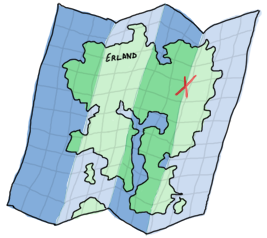
\includegraphics[width=1\linewidth]{erland.png}
\end{wrapfigure}
В начале этой главы я кратко продемонстрировал, как преобразовать две подобные функции в функцию \ops{map/2}.
Также я утверждал, что такую функцию можно использовать для любого списка, в котором мы хотим производить какое\--либо действие с каждым элементом.
Функция выглядела следующим образом:
\begin{lstlisting}[style=erlang]
map(_, []) -> [];
map(F, [H|T]) -> [F(H)|map(F,T)].
\end{lstlisting}
Однако, существует много других абстракций, подобных этой, которые можно построить из часто встречающихся рекурсивных функций.
Давайте для начала взглянем на парочку функций:
\begin{lstlisting}[style=erlang]
%% only keep even numbers
even(L) -> lists:reverse(even(L,[])).
 
even([], Acc) -> Acc;
even([H|T], Acc) when H rem 2 == 0 ->
    even(T, [H|Acc]);
even([_|T], Acc) ->
    even(T, Acc).
 
%% only keep men older than 60
old_men(L) -> lists:reverse(old_men(L,[])).
 
old_men([], Acc) -> Acc;
old_men([Person = {male, Age}|People], Acc) when Age > 60 ->
    old_men(People, [Person|Acc]);
old_men([_|People], Acc) ->
    old_men(People, Acc).
\end{lstlisting}

Первая принимает список чисел и возвращает только чётные.
Вторая проходит по списку с данными вида \{Пол, Возраст\} и возвращает лишь записи о мужчинах старше 60 лет.
В этих функциях найти общее немного сложнее, но некоторое подобие всё же есть.
Обе функции работают над списками, возвращают элементы, которые прошли некий тест (его ещё называют \emph{предикатом}), а остальные элементы отбрасывают.
Из этого обобщения мы можем извлечь всю необходимую нам информацию и преобразовать её в функцию:
\begin{lstlisting}[style=erlang]

filter(Pred, L) -> lists:reverse(filter(Pred, L,[])).
 
filter(_, [], Acc) -> Acc;
filter(Pred, [H|T], Acc) ->
    case Pred(H) of
        true  -> filter(Pred, T, [H|Acc]);
        false -> filter(Pred, T, Acc)
    end.
\end{lstlisting}

Чтобы воспользоваться функцией\--фильтром, нам необходимо лишь получить извне тестирующую функцию.
Скомпилируйте модуль \ops{\href{http://learnyousomeerlang.com/static/erlang/hhfuns.erl}{hhfuns}} и попробуйте им воспользоваться:
\begin{lstlisting}[style=erlang]
1> c(hhfuns).
{ok, hhfuns}
2> Numbers = lists:seq(1,10).
[1,2,3,4,5,6,7,8,9,10]
3> hhfuns:filter(fun(X) -> X rem 2 == 0 end, Numbers).
[2,4,6,8,10]
4> People = [{male,45},{female,67},{male,66},{female,12},{unkown,174},{male,74}].
[{male,45},{female,67},{male,66},{female,12},{unkown,174},{male,74}]
5> hhfuns:filter(fun({Gender,Age}) -> Gender == male andalso Age > 60 end, People).
[{male,66},{male,74}]
\end{lstlisting}

Эти примеры демонстрируют, что программисту, который использует функцию \ops{filter/2}, нужно лишь задать предикат и указать список, который будет фильтроваться.
О самом процессе перемещения по списку и об отбрасывании ненужных элементов думать больше не нужно.
При обобщении функционального кода происходит одна важная вещь: мы пытаемся избавиться от того, что остаётся постоянным, и позволяем программисту предоставить лишь то, что подвергается изменению.

В предыдущей главе мы применяли к спискам другой вид рекурсивных манипуляций, в котором мы последовательно рассматривали каждый элемент списка и приводили их к одному ответу.
Эта операция называется \emph{свёрткой} (fold) и может применяться для следующих функций:
\begin{lstlisting}[style=erlang]
%% find the maximum of a list
max([H|T]) -> max2(T, H).
 
max2([], Max) -> Max;
max2([H|T], Max) when H > Max -> max2(T, H);
max2([_|T], Max) -> max2(T, Max).
 
%% find the minimum of a list
min([H|T]) -> min2(T,H).
 
min2([], Min) -> Min;
min2([H|T], Min) when H < Min -> min2(T,H);
min2([_|T], Min) -> min2(T, Min).
 
%% sum of all the elements of a list
sum(L) -> sum(L,0).
 
sum([], Sum) -> Sum;
sum([H|T], Sum) -> sum(T, H+Sum).
\end{lstlisting}

Чтобы понять как себя ведёт свёртка, нам необходимо найти общее в этих действиях, а после найти различия.
Как было указано выше, мы всегда приводим список к единичному значению.
Следовательно, наша свёртка должна повторять действие, сохраняя один элемент.
Нам не нужно строить новый список.
Стражи нам не понадобятся, так как они присутствуют не всегда, а поэтому должны находиться в пользовательской функции.
В этом отношении наша функция свёртки будет, скорее всего, походить на функцию sum.

\begin{wrapfigure}{r}{0.25\linewidth}
    
\includegraphics[width=1\linewidth]{foldr.png}
\end{wrapfigure}
Ещё одной неприметной частью всех трёх функций, о которой мы пока не упоминали, является то, что у каждой функции должно быть начальное значение, от которого будет начинаться отсчёт.
В случае \ops{sum/2} мы используем 0, так как проводим операцию сложения, которая нейтральна относительно 0, и при вычислении \ops{X = X + 0} мы никак не повлияем на результат.
Если бы мы использовали операцию умножения \ops{X = X * 1}, то в качестве стартового значения избрали бы 1.
У функций \ops{min/1} и \ops{max/1} стартового значения по умолчанию быть не может.
Если список полностью состоит из отрицательных чисел, а мы начнём с 0, то получим неверный результат.
Поэтому нам необходимо использовать в качестве начальной точки первый элемент списка.
К сожалению, мы не можем заранее применить такие рассуждения к любой ситуации, а поэтому оставляем решение этой проблемы программисту.
Принимая во внимание все перечисленные элементы, мы можем построить следующую абстракцию:
\begin{lstlisting}[style=erlang]
fold(_, Start, []) -> Start;
fold(F, Start, [H|T]) -> fold(F, F(H,Start), T).
\end{lstlisting}
А затем исполнить:
\begin{lstlisting}[style=erlang]
6> c(hhfuns).
{ok, hhfuns}
7> [H|T] = [1,7,3,5,9,0,2,3].   
[1,7,3,5,9,0,2,3]
8> hhfuns:fold(fun(A,B) when A > B -> A; (_,B) -> B end, H, T).
9
9> hhfuns:fold(fun(A,B) when A < B -> A; (_,B) -> B end, H, T).
0
10> hhfuns:fold(fun(A,B) -> A + B end, 0, lists:seq(1,6)).
21
\end{lstlisting}

Практически любую функцию, которая сводит список значений к одному элементу, можно выразить в виде свёртки.

Занятно, что вы можете представить аккумулятор как единичный элемент (или единичную переменную), а аккумулятор может быть списком.
Так мы можем использовать свёртку для построения списков.
Это значит, что свёртка универсальна в том смысле, что с её помощью можно реализовать практически любую другую рекурсивную функцию для списков, даже отображение и фильтр:
\begin{lstlisting}[style=erlang]
reverse(L) ->
    fold(fun(X,Acc) -> [X|Acc] end, [], L).
 
map2(F,L) ->
    reverse(fold(fun(X,Acc) -> [F(X)|Acc] end, [], L)).
 
filter2(Pred, L) ->
    F = fun(X,Acc) ->
        case Pred(X) of
            true  -> [X|Acc];
            false -> Acc
        end
    end,
    reverse(fold(F, [], L)).
\end{lstlisting}

И эти функции будут работать так же как и те, что мы написали ранее.
Ну как, мощные абстракции или нет?

Отображение, фильтры и свёртки \--- это лишь часть функций для списков, которые предоставляются стандартной библиотекой Erlang (см. \ops{\href{http://erldocs.com/R15B/stdlib/lists.html\#map/2}{lists:map/2}}, \ops{\href{http://erldocs.com/R15B/stdlib/lists.html\#filter/2}{lists:filter/2}}, \ops{\href{http://erldocs.com/R15B/stdlib/lists.html\#foldl/3}{lists:foldl/3}} и \ops{\href{http://erldocs.com/R15B/stdlib/lists.html\#foldr/3}{lists:foldr/3}}.
Стоит отметить также функции \ops{\href{http://erldocs.com/R15B/stdlib/lists.html\#all/2}{all/2}} и \ops{\href{http://erldocs.com/R15B/stdlib/lists.html\#any/2}{any/2}}, которые принимают предикат и проверяют, что для каждого элемента предикат возвращает true, или что хотя бы для одного из них предикат возвращает true, соответственно.
Ещё есть функция \ops{\href{http://erldocs.com/R15B/stdlib/lists.html\#dropwhile/2}{dropwhile/2}}, которая игнорирует элементы списка до тех пор, пока не находит один, удовлетворяющий предикату, и противоположная функция \ops{\href{http://erldocs.com/R15B/stdlib/lists.html\#takewhile/2}{takewhile/2}}, которая будет возвращать элементы до тех пор, пока не встретит такой, для которого предикат не возвращает true.
Две предыдущие функции объединяет \ops{\href{http://erldocs.com/R15B/stdlib/lists.html\#partition/2}{partition/2}}.
Эта функция принимает один список, а возвращает два.
Первый содержит термы, которые удовлетворяют предикату, а второй \--- остальные элементы. Кроме того, для обработки списков часто используются такие функции как \ops{\href{http://erldocs.com/R15B/stdlib/lists.html\#flatten/1}{flatten/1}}, \ops{\href{http://erldocs.com/R15B/stdlib/lists.html\#flatlength/1}{flatlength/1}}, \ops{\href{http://erldocs.com/R15B/stdlib/lists.html\#flatmap/2}{flatmap/2}}, \ops{\href{http://erldocs.com/R15B/stdlib/lists.html\#merge/1}{merge/1}}, \ops{\href{http://erldocs.com/R15B/stdlib/lists.html\#nth/2}{nth/2}}, \ops{\href{http://erldocs.com/R15B/stdlib/lists.html\#nthtail/2}{nthtail/2}}, \ops{\href{http://erldocs.com/R15B/stdlib/lists.html\#split/2}{split/2}} и другие.

Также в этом модуле можно найти и другие функции, такие как zip\--функция (которую мы рассматривали в предыдущей главе), unzip\--функция, комбинации отображений и свёрток и т.д.
Рекомендую вам прочитать \href{http://erldocs.com/R15B/stdlib/lists.html}{описание списков}.
В этом документе вы найдёте примеры использования списковых функций.
Применяя те концепции, которые были заключены умными людьми в этих абстракциях, у вас редко будет появляться необходимость в самостоятельном создании рекурсивных функций.
